\documentclass{article}\usepackage[]{graphicx}\usepackage[]{color}
% maxwidth is the original width if it is less than linewidth
% otherwise use linewidth (to make sure the graphics do not exceed the margin)
\makeatletter
\def\maxwidth{ %
  \ifdim\Gin@nat@width>\linewidth
    \linewidth
  \else
    \Gin@nat@width
  \fi
}
\makeatother

\definecolor{fgcolor}{rgb}{0.345, 0.345, 0.345}
\newcommand{\hlnum}[1]{\textcolor[rgb]{0.686,0.059,0.569}{#1}}%
\newcommand{\hlstr}[1]{\textcolor[rgb]{0.192,0.494,0.8}{#1}}%
\newcommand{\hlcom}[1]{\textcolor[rgb]{0.678,0.584,0.686}{\textit{#1}}}%
\newcommand{\hlopt}[1]{\textcolor[rgb]{0,0,0}{#1}}%
\newcommand{\hlstd}[1]{\textcolor[rgb]{0.345,0.345,0.345}{#1}}%
\newcommand{\hlkwa}[1]{\textcolor[rgb]{0.161,0.373,0.58}{\textbf{#1}}}%
\newcommand{\hlkwb}[1]{\textcolor[rgb]{0.69,0.353,0.396}{#1}}%
\newcommand{\hlkwc}[1]{\textcolor[rgb]{0.333,0.667,0.333}{#1}}%
\newcommand{\hlkwd}[1]{\textcolor[rgb]{0.737,0.353,0.396}{\textbf{#1}}}%
\let\hlipl\hlkwb

\usepackage{framed}
\makeatletter
\newenvironment{kframe}{%
 \def\at@end@of@kframe{}%
 \ifinner\ifhmode%
  \def\at@end@of@kframe{\end{minipage}}%
  \begin{minipage}{\columnwidth}%
 \fi\fi%
 \def\FrameCommand##1{\hskip\@totalleftmargin \hskip-\fboxsep
 \colorbox{shadecolor}{##1}\hskip-\fboxsep
     % There is no \\@totalrightmargin, so:
     \hskip-\linewidth \hskip-\@totalleftmargin \hskip\columnwidth}%
 \MakeFramed {\advance\hsize-\width
   \@totalleftmargin\z@ \linewidth\hsize
   \@setminipage}}%
 {\par\unskip\endMakeFramed%
 \at@end@of@kframe}
\makeatother

\definecolor{shadecolor}{rgb}{.97, .97, .97}
\definecolor{messagecolor}{rgb}{0, 0, 0}
\definecolor{warningcolor}{rgb}{1, 0, 1}
\definecolor{errorcolor}{rgb}{1, 0, 0}
\newenvironment{knitrout}{}{} % an empty environment to be redefined in TeX

\usepackage{alltt}
\usepackage[sc]{mathpazo}
\renewcommand{\sfdefault}{lmss}
\renewcommand{\ttdefault}{lmtt}
\usepackage[T1]{fontenc}
\usepackage{geometry}
\geometry{verbose,tmargin=2.5cm,bmargin=2.5cm,lmargin=2.5cm,rmargin=2.5cm}
\setcounter{secnumdepth}{2}
\setcounter{tocdepth}{2}
\usepackage[unicode=true,pdfusetitle,
 bookmarks=true,bookmarksnumbered=true,bookmarksopen=true,bookmarksopenlevel=2,
 breaklinks=false,pdfborder={0 0 1},backref=false,colorlinks=false]
 {hyperref}
\hypersetup{
 pdfstartview={XYZ null null 1}}

\makeatletter
%%%%%%%%%%%%%%%%%%%%%%%%%%%%%% User specified LaTeX commands.
\renewcommand{\textfraction}{0.05}
\renewcommand{\topfraction}{0.8}
\renewcommand{\bottomfraction}{0.8}
\renewcommand{\floatpagefraction}{0.75}

\makeatother
\IfFileExists{upquote.sty}{\usepackage{upquote}}{}
\begin{document}









\begin{knitrout}
\definecolor{shadecolor}{rgb}{0.969, 0.969, 0.969}\color{fgcolor}\begin{kframe}
\begin{alltt}
\hlcom{#### PROBABILIDAD Y ESTADÍSTICA FUNDAMENTAL  #####}
\hlcom{###################  PARCIAL 3  ###################}
\hlcom{#}
\hlcom{# Wullfredo Javier Barco Godoy}
\hlcom{# Ángela Zoraya Cortés Yepes}
\hlcom{# Juan Manuel Garcia Mejia}
\hlcom{# Andrés Felipe Patiño Nivia}
\hlcom{# Jafeth Paz Cortés}
\hlcom{#}
\hlcom{###################################################}


\hlcom{# 1 - Saturación de gas residual}
\hlstd{m1} \hlkwb{<-} \hlkwd{c}\hlstd{(}\hlnum{23.5}\hlstd{,} \hlnum{31.5}\hlstd{,} \hlnum{34.0}\hlstd{,} \hlnum{46.7}\hlstd{,} \hlnum{45.6}\hlstd{,} \hlnum{32.5}\hlstd{,} \hlnum{41.4}\hlstd{,} \hlnum{37.2}\hlstd{,} \hlnum{42.5}\hlstd{,}
        \hlnum{46.9}\hlstd{,} \hlnum{51.5}\hlstd{,} \hlnum{36.4}\hlstd{,} \hlnum{44.5}\hlstd{,} \hlnum{35.7}\hlstd{,} \hlnum{33.5}\hlstd{,} \hlnum{39.3}\hlstd{,} \hlnum{22.0}\hlstd{,} \hlnum{51.2}\hlstd{)}

\hlkwd{qqnorm}\hlstd{(m1,} \hlkwc{main}\hlstd{=}\hlstr{"QQ plot de una normal"}\hlstd{);} \hlkwd{qqline}\hlstd{(m1)} \hlcom{# Gráfico de normalidad}
\end{alltt}
\end{kframe}

{\centering 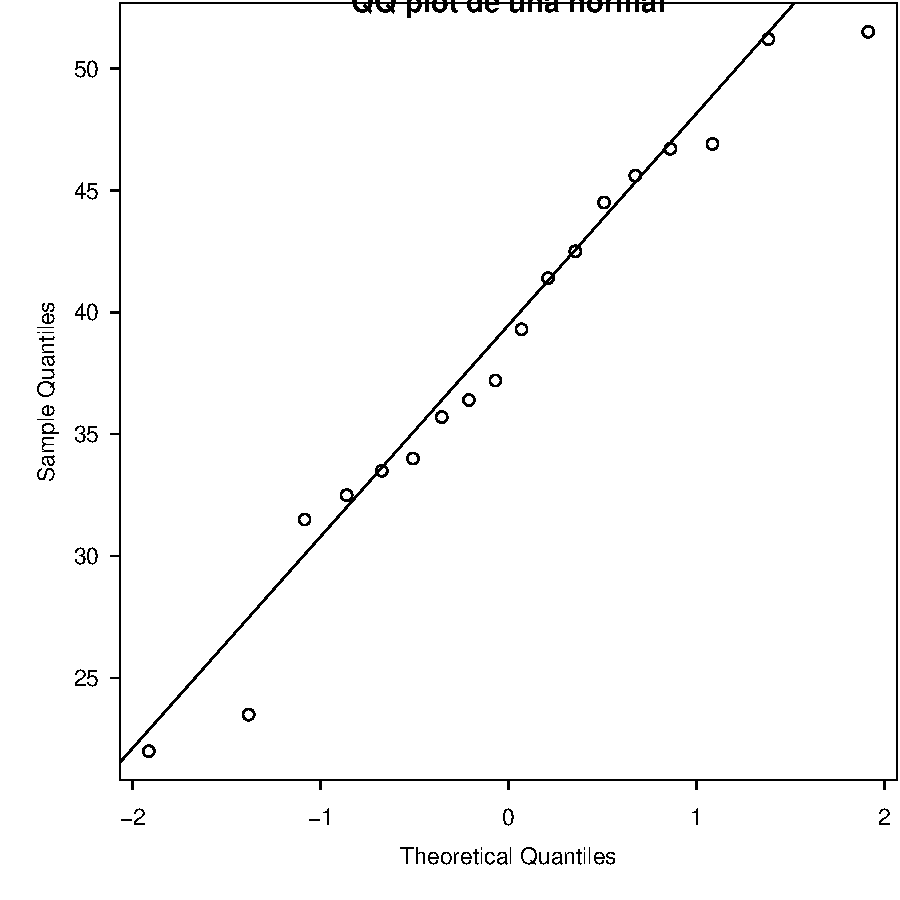
\includegraphics[width=.6\linewidth]{figure/Parcial-3-Rnwauto-report-1} 

}


\begin{kframe}\begin{alltt}
\hlstd{s_mu} \hlkwb{<-} \hlkwd{sd}\hlstd{(m1)} \hlcom{# Desv estandar}
\hlstd{n} \hlkwb{<-} \hlkwd{length}\hlstd{(m1)} \hlcom{# Cantidad de datos}
\hlstd{prom} \hlkwb{<-} \hlkwd{mean}\hlstd{(m1)} \hlcom{# Promedio}

\hlstd{t_crit} \hlkwb{<-} \hlkwd{round}\hlstd{(}\hlkwd{qt}\hlstd{(}\hlkwd{c}\hlstd{(}\hlnum{0.025}\hlstd{),}\hlkwc{df} \hlstd{= n}\hlopt{-}\hlnum{1}\hlstd{,}\hlkwc{lower.tail} \hlstd{= F),}\hlnum{3}\hlstd{)}
\hlstd{LI_mu} \hlkwb{<-} \hlkwd{round}\hlstd{(prom} \hlopt{-} \hlstd{t_crit}\hlopt{*}\hlstd{s_mu}\hlopt{/}\hlkwd{sqrt}\hlstd{(n),}\hlnum{3}\hlstd{)}
\hlstd{LS_mu} \hlkwb{<-} \hlkwd{round}\hlstd{(prom} \hlopt{+} \hlstd{t_crit}\hlopt{*}\hlstd{s_mu}\hlopt{/}\hlkwd{sqrt}\hlstd{(n),}\hlnum{3}\hlstd{)}

\hlkwd{paste}\hlstd{(}\hlstr{"El intervalo de confianza para mu del 95% es:"}\hlstd{,LI_mu,LS_mu)}
\end{alltt}
\begin{verbatim}
## [1] "El intervalo de confianza para mu del 95% es: 34.447 42.875"
\end{verbatim}
\begin{alltt}
\hlkwd{t.test}\hlstd{(}\hlkwc{x} \hlstd{= m1,} \hlkwc{y} \hlstd{=} \hlkwa{NULL}\hlstd{,}\hlkwc{alternative} \hlstd{=} \hlstr{"two.sided"}\hlstd{,} \hlkwc{conf.level} \hlstd{=} \hlnum{0.95}\hlstd{)} \hlcom{# El método que se utilizó en realidad}
\end{alltt}
\begin{verbatim}
## 
## 	One Sample t-test
## 
## data:  m1
## t = 19.358, df = 17, p-value = 5.097e-13
## alternative hypothesis: true mean is not equal to 0
## 95 percent confidence interval:
##  34.44748 42.87474
## sample estimates:
## mean of x 
##  38.66111
\end{verbatim}
\begin{alltt}
\hlcom{# 2 - Medios inalambricos}
\hlstd{x2} \hlkwb{=} \hlnum{1262}\hlstd{; n2} \hlkwb{=} \hlnum{2253}

\hlkwd{prop.test}\hlstd{(}\hlkwc{x}\hlstd{=}\hlnum{1262}\hlstd{,} \hlkwc{n}\hlstd{=}\hlnum{2253}\hlstd{,} \hlkwc{conf.level}\hlstd{=}\hlnum{0.95}\hlstd{)}\hlopt{$}\hlstd{conf.int}
\end{alltt}
\begin{verbatim}
## [1] 0.5393380 0.5807391
## attr(,"conf.level")
## [1] 0.95
\end{verbatim}
\begin{alltt}
\hlcom{# 3 - Pasajeros de aerolinea}
\hlstd{Pasajeros} \hlkwb{<-} \hlkwd{c}\hlstd{(}\hlnum{163}\hlstd{,} \hlnum{165}\hlstd{,} \hlnum{094}\hlstd{,} \hlnum{137}\hlstd{,} \hlnum{123}\hlstd{,} \hlnum{095}\hlstd{,} \hlnum{170}\hlstd{,} \hlnum{096}\hlstd{,} \hlnum{117}\hlstd{,} \hlnum{129}\hlstd{,}
               \hlnum{152}\hlstd{,} \hlnum{138}\hlstd{,} \hlnum{147}\hlstd{,} \hlnum{119}\hlstd{,} \hlnum{166}\hlstd{,} \hlnum{125}\hlstd{,} \hlnum{148}\hlstd{,} \hlnum{180}\hlstd{,} \hlnum{152}\hlstd{,} \hlnum{149}\hlstd{,}
               \hlnum{167}\hlstd{,} \hlnum{120}\hlstd{,} \hlnum{129}\hlstd{,} \hlnum{159}\hlstd{,} \hlnum{150}\hlstd{,} \hlnum{119}\hlstd{,} \hlnum{113}\hlstd{,} \hlnum{147}\hlstd{,} \hlnum{169}\hlstd{,} \hlnum{151}\hlstd{,}
               \hlnum{116}\hlstd{,} \hlnum{150}\hlstd{,} \hlnum{110}\hlstd{,} \hlnum{110}\hlstd{,} \hlnum{143}\hlstd{,} \hlnum{090}\hlstd{,} \hlnum{134}\hlstd{,} \hlnum{145}\hlstd{,} \hlnum{156}\hlstd{,} \hlnum{165}\hlstd{,}
               \hlnum{174}\hlstd{,} \hlnum{133}\hlstd{,} \hlnum{128}\hlstd{,} \hlnum{100}\hlstd{,} \hlnum{086}\hlstd{,} \hlnum{148}\hlstd{,} \hlnum{139}\hlstd{,} \hlnum{150}\hlstd{,} \hlnum{145}\hlstd{,} \hlnum{100}\hlstd{)}

\hlkwd{mean}\hlstd{(Pasajeros)} \hlcom{# utilizamos Z= (X-x)/s ~N(0,1)}
\end{alltt}
\begin{verbatim}
## [1] 136.22
\end{verbatim}
\begin{alltt}
\hlkwd{t.test}\hlstd{(Pasajeros,}\hlkwc{conf.level} \hlstd{=} \hlnum{0.95}\hlstd{)}
\end{alltt}
\begin{verbatim}
## 
## 	One Sample t-test
## 
## data:  Pasajeros
## t = 39.413, df = 49, p-value < 2.2e-16
## alternative hypothesis: true mean is not equal to 0
## 95 percent confidence interval:
##  129.2744 143.1656
## sample estimates:
## mean of x 
##    136.22
\end{verbatim}
\begin{alltt}
\hlcom{# 4 - Ruptura de circuitos electricamente sobrecargados}
\hlstd{datosenunciado}\hlkwb{<-}\hlkwd{c}\hlstd{(}\hlnum{1470}\hlstd{,} \hlnum{1510}\hlstd{,} \hlnum{1690}\hlstd{,} \hlnum{1740}\hlstd{,} \hlnum{1900}\hlstd{,} \hlnum{2000}\hlstd{,} \hlnum{2030}\hlstd{,} \hlnum{2100}\hlstd{,} \hlnum{2190}\hlstd{,} \hlnum{2200}\hlstd{,}
                  \hlnum{2290}\hlstd{,} \hlnum{2380}\hlstd{,} \hlnum{2390}\hlstd{,}  \hlnum{2480}\hlstd{,} \hlnum{2500}\hlstd{,} \hlnum{2580}\hlstd{,} \hlnum{2700}\hlstd{)}
\hlkwd{mean}\hlstd{(datosenunciado)}
\end{alltt}
\begin{verbatim}
## [1] 2126.471
\end{verbatim}
\begin{alltt}
\hlstd{media}\hlkwb{<-}\hlkwd{mean}\hlstd{(datosenunciado)}
\hlstd{z}\hlkwb{<-} \hlnum{1.96}
\hlkwd{length}\hlstd{(datosenunciado)}
\end{alltt}
\begin{verbatim}
## [1] 17
\end{verbatim}
\begin{alltt}
\hlstd{n}\hlkwb{<-} \hlkwd{length}\hlstd{(datosenunciado)}
\hlkwd{sd}\hlstd{(datosenunciado)}
\end{alltt}
\begin{verbatim}
## [1] 370.5729
\end{verbatim}
\begin{alltt}
\hlstd{desviacion}\hlkwb{<-}\hlstd{(}\hlkwd{sd}\hlstd{(datosenunciado))}
\hlstd{errorestandar}\hlkwb{<-} \hlstd{desviacion}\hlopt{/}\hlkwd{sqrt}\hlstd{(n)}
\hlstd{lim_inf}\hlkwb{<-}\hlstd{media}\hlopt{-}\hlstd{(z}\hlopt{*}\hlstd{errorestandar)}
\hlstd{lim_sup}\hlkwb{<-}\hlstd{media}\hlopt{+}\hlstd{(z}\hlopt{*}\hlstd{errorestandar)}
\hlstd{resultado}\hlkwb{<-} \hlkwd{data.frame}\hlstd{(n, desviacion, errorestandar, lim_inf, lim_sup)}


\hlcom{# 5 - Visita de animales domesticos al veterinario en un a<U+663C><U+3E31>o}
\hlstd{media}\hlkwb{<-}\hlnum{3.59}
\hlstd{desviacion}\hlkwb{<-}\hlnum{1.045}
\hlstd{x_1}\hlkwb{<-}\hlnum{3.49}
\hlstd{x_2}\hlkwb{<-}\hlnum{3.69}
\hlstd{z}\hlkwb{<-}\hlstd{(x_2}\hlopt{-}\hlstd{media)}\hlopt{/}\hlstd{desviacion} \hlcom{# el valor que buscamos en la tabla }
  \hlcom{# si a+IC=53.59 entonces }
  \hlstd{b}\hlkwb{<-}\hlnum{46.41} \hlcom{# en consecuencia,}
  \hlstd{a}\hlkwb{<-}\hlnum{46.41}
\hlstd{porcentajedeintervalodeconfianza}\hlkwb{<-}\hlnum{100}\hlopt{-}\hlstd{a}\hlopt{-}\hlstd{b} \hlcom{# el porcentaje de este intervalo es 7.18}


\hlcom{# 6 - Asbesto y elasticidad pulmonar}
\hlstd{m6} \hlkwb{<-} \hlkwd{c}\hlstd{(}\hlnum{167.9}\hlstd{,} \hlnum{180.8}\hlstd{,} \hlnum{184.8}\hlstd{,} \hlnum{189.8}\hlstd{,} \hlnum{194.8}\hlstd{,} \hlnum{200.2}\hlstd{,} \hlnum{201.9}\hlstd{,} \hlnum{206.9}\hlstd{,}
        \hlnum{207.2}\hlstd{,} \hlnum{208.4}\hlstd{,} \hlnum{226.3}\hlstd{,} \hlnum{227.7}\hlstd{,} \hlnum{228.5}\hlstd{,} \hlnum{232.4}\hlstd{,} \hlnum{239.8}\hlstd{,} \hlnum{258.6}\hlstd{)}

\hlkwd{t.test}\hlstd{(}\hlkwc{x} \hlstd{= m6,} \hlkwc{y} \hlstd{=} \hlkwa{NULL}\hlstd{,}\hlkwc{alternative} \hlstd{=} \hlstr{"two.sided"}\hlstd{,} \hlkwc{conf.level} \hlstd{=} \hlnum{0.99}\hlstd{)}
\end{alltt}
\begin{verbatim}
## 
## 	One Sample t-test
## 
## data:  m6
## t = 34.732, df = 15, p-value = 9.516e-16
## alternative hypothesis: true mean is not equal to 0
## 99 percent confidence interval:
##  191.9547 227.5453
## sample estimates:
## mean of x 
##    209.75
\end{verbatim}
\begin{alltt}
\hlkwd{qqnorm}\hlstd{(m6,} \hlkwc{main}\hlstd{=}\hlstr{"QQ plot de una normal"}\hlstd{)}
\hlkwd{qqline}\hlstd{(m6)}
\end{alltt}
\end{kframe}

{\centering 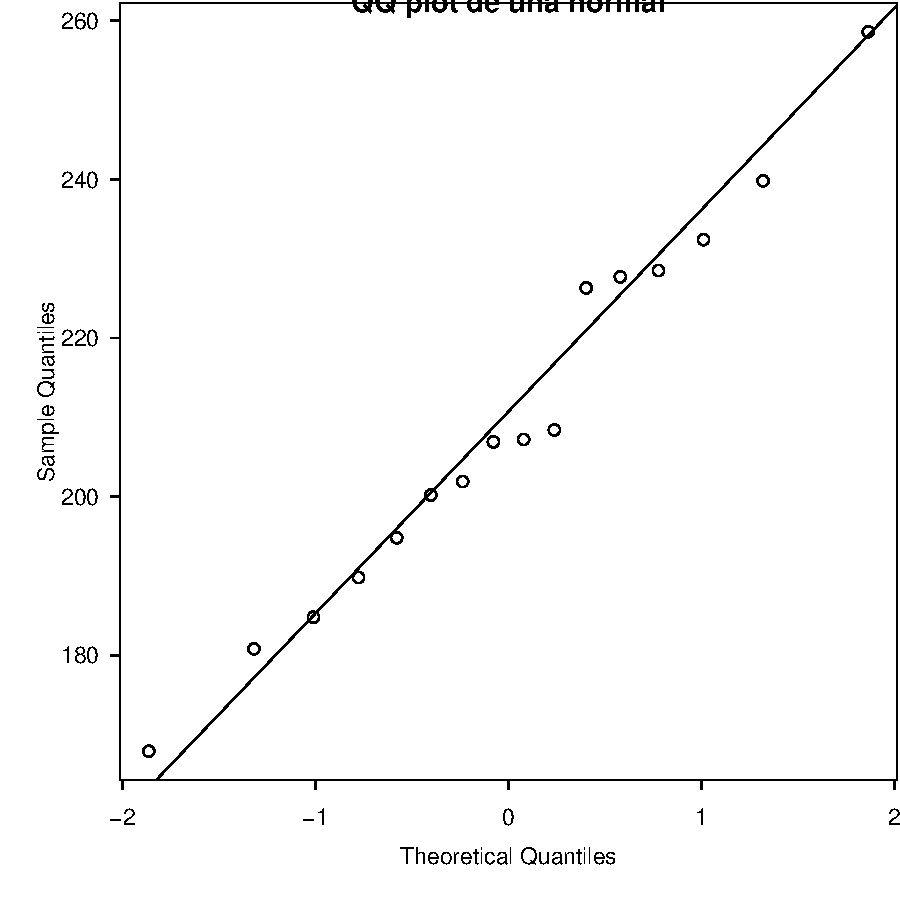
\includegraphics[width=.6\linewidth]{figure/Parcial-3-Rnwauto-report-2} 

}


\begin{kframe}\begin{alltt}
\hlcom{# 7 - Secado de pintura}
\hlstd{B} \hlkwb{=} \hlkwd{c}\hlstd{(}\hlnum{2.8}\hlstd{,}\hlnum{3.3}\hlstd{,}\hlnum{5.6}\hlstd{,}\hlnum{3.7}\hlstd{,}\hlnum{2.8}\hlstd{,}\hlnum{4.4}\hlstd{,}\hlnum{4.0}\hlstd{,}\hlnum{5.2}\hlstd{,}\hlnum{3.0}\hlstd{,}\hlnum{4.8}\hlstd{,}\hlnum{3.4}\hlstd{,}\hlnum{2.5}\hlstd{,}\hlnum{4.8}\hlstd{,}\hlnum{2.9}\hlstd{,}\hlnum{3.6}\hlstd{)}

\hlkwd{boxplot}\hlstd{(B,}\hlkwc{horizontal} \hlstd{= T)}
\end{alltt}
\end{kframe}

{\centering 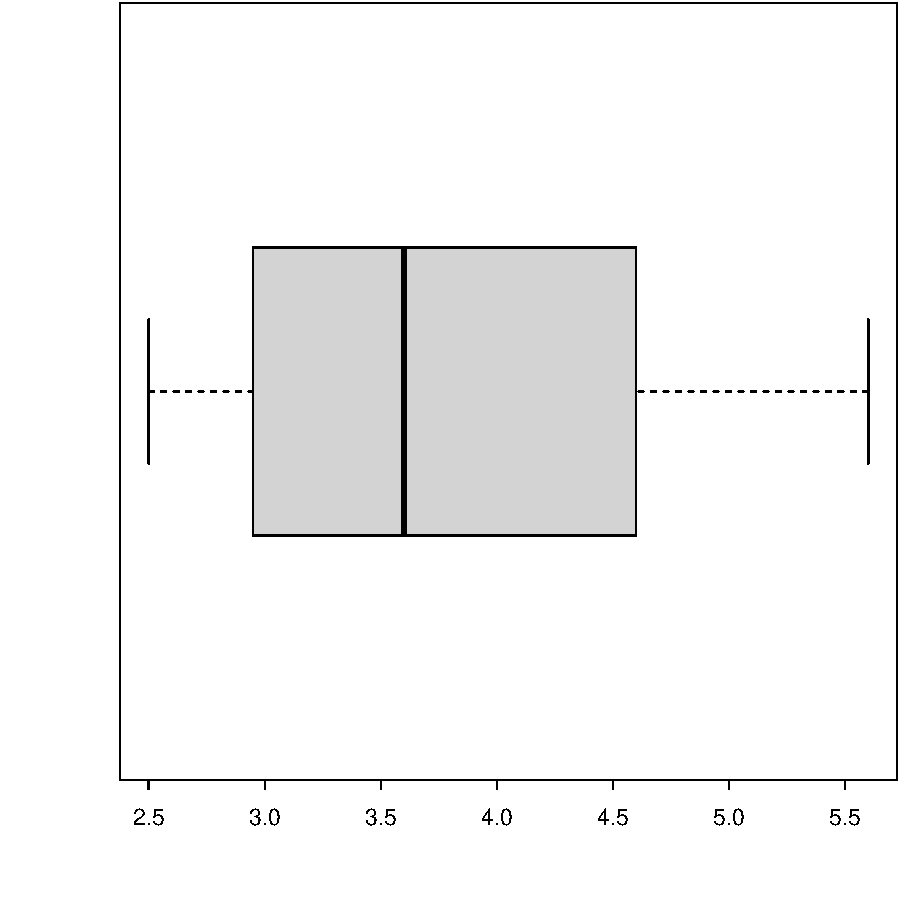
\includegraphics[width=.6\linewidth]{figure/Parcial-3-Rnwauto-report-3} 

}


\begin{kframe}\begin{alltt}
\hlkwd{t.test}\hlstd{(}\hlkwc{x} \hlstd{=B,}\hlkwc{conf.level} \hlstd{=} \hlnum{0.95}\hlstd{)}\hlopt{$}\hlstd{conf.int}
\end{alltt}
\begin{verbatim}
## [1] 3.248995 4.324339
## attr(,"conf.level")
## [1] 0.95
\end{verbatim}
\begin{alltt}
\hlcom{# 8 - Conjetura}
\hlcom{# n=(z^2??/2)/4e^2}
\hlcom{# Z??/2= Z0.005= 2.575}
\hlstd{e} \hlkwb{<-} \hlnum{0.01}
\hlstd{z} \hlkwb{<-} \hlnum{2.575}
\hlstd{n} \hlkwb{<-}\hlstd{(z}\hlopt{^}\hlnum{2}\hlstd{)}\hlopt{/}\hlstd{(}\hlnum{4}\hlopt{*}\hlstd{(e}\hlopt{^}\hlnum{2}\hlstd{)); n}
\end{alltt}
\begin{verbatim}
## [1] 16576.56
\end{verbatim}
\begin{alltt}
\hlcom{# 9 - Dureza de Rockwell en cabeza de alfileres}
\hlstd{d_rockwell} \hlkwb{<-} \hlkwd{c}\hlstd{(}\hlnum{48.68}\hlstd{,} \hlnum{48.70}\hlstd{,} \hlnum{47.69}\hlstd{,} \hlnum{46.23}\hlstd{,}
                \hlnum{50.45}\hlstd{,} \hlnum{48.61}\hlstd{,} \hlnum{48.16}\hlstd{,} \hlnum{49.44}\hlstd{,}
                \hlnum{47.29}\hlstd{,} \hlnum{48.58}\hlstd{,} \hlnum{48.92}\hlstd{,} \hlnum{46.79}\hlstd{)}

\hlkwd{t.test}\hlstd{(}\hlkwc{x}\hlstd{=d_rockwell,} \hlkwc{conf.level} \hlstd{=} \hlnum{0.90}\hlstd{)}\hlopt{$}\hlstd{conf.int}
\end{alltt}
\begin{verbatim}
## [1] 47.69443 48.89557
## attr(,"conf.level")
## [1] 0.9
\end{verbatim}
\begin{alltt}
\hlcom{# 10 - Rockwell, parte 2}
\hlstd{n} \hlkwb{<-} \hlkwd{length}\hlstd{(d_rockwell)}
\hlstd{s} \hlkwb{<-} \hlkwd{sd}\hlstd{(d_rockwell)}

\hlstd{chi_derecha} \hlkwb{<-} \hlkwd{round}\hlstd{(}\hlkwd{qchisq}\hlstd{(}\hlkwd{c}\hlstd{(}\hlnum{0.021}\hlstd{),}\hlkwc{df} \hlstd{= n}\hlopt{-}\hlnum{1}\hlstd{,}\hlkwc{lower.tail} \hlstd{= F),}\hlnum{3}\hlstd{)}
\hlstd{chi_izquierda} \hlkwb{<-} \hlkwd{round}\hlstd{(}\hlkwd{qchisq}\hlstd{(}\hlkwd{c}\hlstd{(}\hlnum{0.021}\hlstd{),}\hlkwc{df} \hlstd{= n}\hlopt{-}\hlnum{1}\hlstd{,}\hlkwc{lower.tail} \hlstd{= T),}\hlnum{3}\hlstd{)}

\hlstd{LI_scuad} \hlkwb{=} \hlstd{(n}\hlopt{-}\hlnum{1}\hlstd{)}\hlopt{*}\hlstd{s}\hlopt{^}\hlnum{2}\hlopt{/}\hlstd{chi_derecha}
\hlstd{LI_ds} \hlkwb{=} \hlkwd{round}\hlstd{(}\hlkwd{sqrt}\hlstd{(LI_scuad),}\hlnum{4}\hlstd{)}
\hlstd{LS_scuad} \hlkwb{=} \hlstd{(n}\hlopt{-}\hlnum{1}\hlstd{)}\hlopt{*}\hlstd{s}\hlopt{^}\hlnum{2}\hlopt{/}\hlstd{chi_izquierda}
\hlstd{LS_ds} \hlkwb{=} \hlkwd{round}\hlstd{(}\hlkwd{sqrt}\hlstd{(LS_scuad),}\hlnum{4}\hlstd{)}

\hlkwd{paste}\hlstd{(}\hlstr{"El intervalo de confianza para la desviacion est<U+653C><U+3E31>ndar del 99% es:"}\hlstd{,LI_ds,LS_ds)}
\end{alltt}
\begin{verbatim}
## [1] "El intervalo de confianza para la desviacion est<U+653C><U+3E31>ndar del 99% es: 0.8106 2.0102"
\end{verbatim}
\end{kframe}
\end{knitrout}

The R session information (including the OS info, R version and all
packages used):

\begin{knitrout}
\definecolor{shadecolor}{rgb}{0.969, 0.969, 0.969}\color{fgcolor}\begin{kframe}
\begin{alltt}
\hlkwd{sessionInfo}\hlstd{()}
\end{alltt}
\begin{verbatim}
## R version 4.1.1 (2021-08-10)
## Platform: x86_64-w64-mingw32/x64 (64-bit)
## Running under: Windows 10 x64 (build 22000)
## 
## Matrix products: default
## 
## locale:
## [1] LC_COLLATE=Spanish_Spain.1252  LC_CTYPE=Spanish_Spain.1252   
## [3] LC_MONETARY=Spanish_Spain.1252 LC_NUMERIC=C                  
## [5] LC_TIME=Spanish_Spain.1252    
## 
## attached base packages:
## [1] stats     graphics  grDevices utils     datasets  methods   base     
## 
## loaded via a namespace (and not attached):
##  [1] compiler_4.1.1  fastmap_1.1.0   magrittr_2.0.1  htmltools_0.5.2 tools_4.1.1    
##  [6] yaml_2.2.1      stringi_1.7.5   rmarkdown_2.11  highr_0.9       knitr_1.36     
## [11] forcats_0.5.1   stringr_1.4.0   xfun_0.26       digest_0.6.28   rlang_0.4.11   
## [16] evaluate_0.14
\end{verbatim}
\begin{alltt}
\hlkwd{Sys.time}\hlstd{()}
\end{alltt}
\begin{verbatim}
## [1] "2022-01-26 17:29:10 -05"
\end{verbatim}
\end{kframe}
\end{knitrout}


\end{document}
